\documentclass[9pt]{beamer}

\usepackage{appendixnumberbeamer}
\usepackage{booktabs}
\usepackage[scale=2]{ccicons}
\usepackage{pgfplots}
\usepackage{tikz}
\usepackage{graphics}
\usepackage{soul}

\usepgfplotslibrary{dateplot}
\pdfstringdefDisableCommands{\def\translate#1{#1}}
\geometry{paperwidth=140mm, paperheight=105mm}
\usetheme{metropolis}
\bibliographystyle{abbrv}
\setbeamertemplate{frame footer}{Metamaterials and Metastructures}

\usetikzlibrary{shapes, arrows}
\tikzstyle{startstop} = [rectangle, rounded corners, minimum width=2cm, minimum height=1cm, text centered, draw=black, fill=red!30]
\tikzstyle{io} = [trapezium, trapezium stretches=true, trapezium left angle=70, trapezium right angle=110, minimum width=2cm, minimum height=1cm, text centered, draw=black, fill=blue!30]
\tikzstyle{process} = [rectangle, minimum width=2cm, minimum height=1cm, text centered, text width=2cm, draw=black, fill=orange!30]
\tikzstyle{decision} = [diamond, minimum width=2cm, minimum height=1cm, text centered, draw=black, fill=green!30]
\tikzstyle{arrow} = [thick,->,>=stealth]

\title{Study on Nonreciprocal Behavior in Time-Space Modulated Beams}
\subtitle{Control of structural band-gaps via shunted piezoelectric patches}
\date{12/02/2025}
\author{Tommaso Bocchietti 10740309 \\ Konstantinos Georgoussis 10992540 \\ (Luciano Sarri 11071336)}
\institute{Politecnico di Milano}
\titlegraphic{\hfill
\includegraphics[height=1.5cm]{pdf/Polimi_logo_header.pdf}}

\begin{document}

\maketitle

\begin{frame}{Agenda}

    \begin{columns}[c, onlytextwidth]

        \begin{column}{0.4\textwidth}

            \setbeamertemplate{section in toc}[sections numbered]
            \tableofcontents

        \end{column}

        \begin{column}{0.6\textwidth}

            \begin{figure}[H]
                \centering
                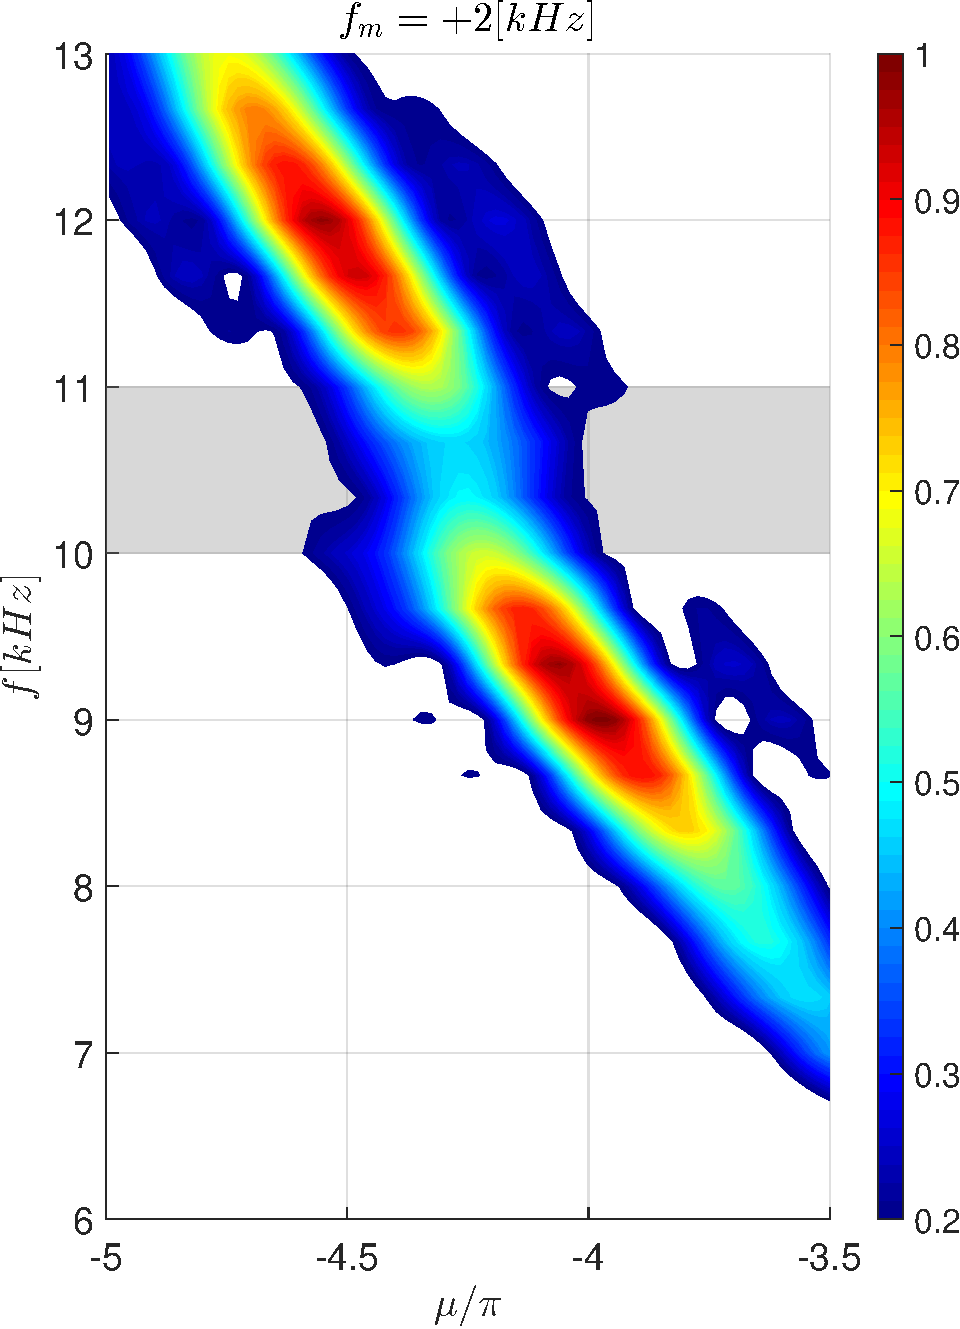
\includegraphics[width=0.48\textwidth]{img/MATLAB/EXP_nonreciprocal_@+2kHz.pdf}
                \hfill
                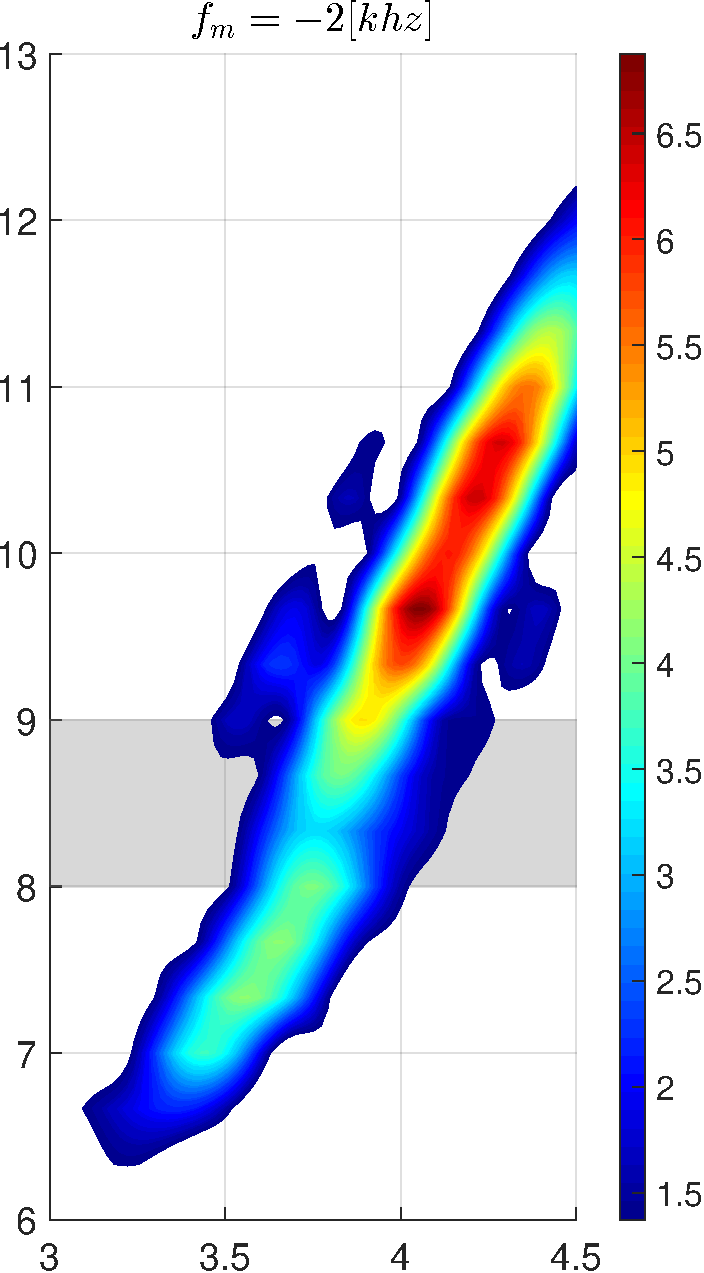
\includegraphics[width=0.48\textwidth]{img/MATLAB/EXP_nonreciprocal_@-2kHz.pdf}
                \caption{\hl{Re-export with label on axis}}
            \end{figure}

        \end{column}

    \end{columns}

\end{frame}


% - The idea of shunted piezo connect to piezo == modulation in the beam properties (theoretical part)
% - Sensitivity analysis
% - Experimental results for space modulation only
% - Experimental result for also time modulated and focus on nonreciprocity

% \section{Introduction}


\begin{frame}{Introduction to nonreciprocity}

    The principle of reciprocity states that the in a linear time-invariant system (LTI), waves propagate from $A$ to $B$ in the same way as from $B$ to $A$.
    The violation of this principle is referred to as \textbf{nonreciprocal} behavior.

    \vspace{9pt}

    One question arise: \textbf{is it possible to design a system that achieves nonreciprocal behavior?}

    % Breaking reciprocity in wave propagation enables the development of one-way communication devices with enhanced performance.

\end{frame}



\begin{frame}{Experimental setup}

    The experimental setup\footnotemark[1] is composed of an array of shunted piezoelectric patches spaced $2$ mm apart placed on an aluminum beam substrate.
    Toggling the switches that control the connection between the power supply and each negative capacitance shunting circuit, allows to modulate the substrate properties.

    \begin{figure}[H]
        \centering
        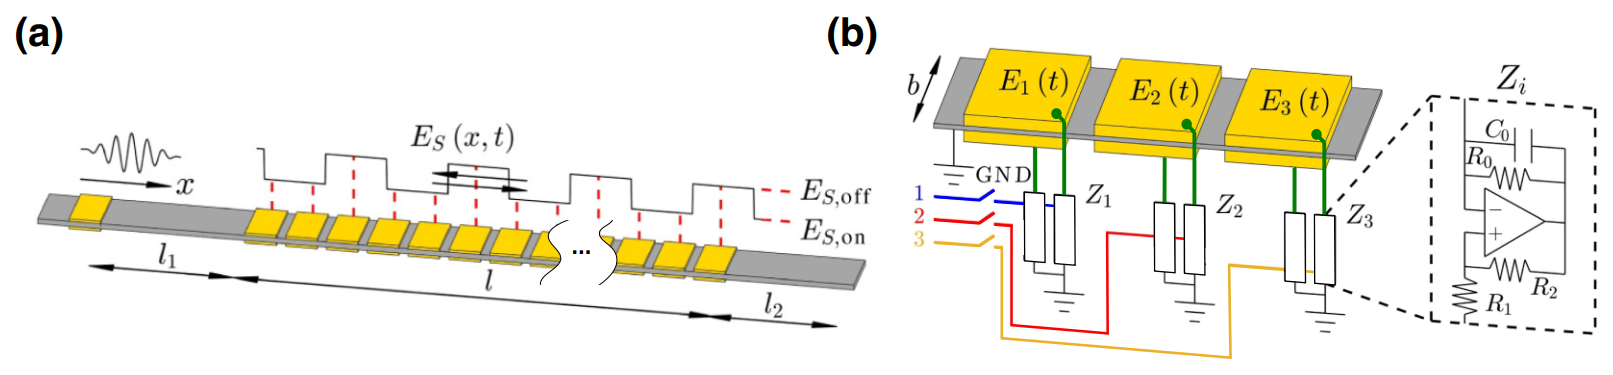
\includegraphics[width=0.9\textwidth]{img/experimental_setup_scheme.png}
        \caption{Beam substrate and array of piezoelectric patches (a), Spatio-Temporal cell and shunting circuits (b).}
    \end{figure}

    Out-of-plane velocity field is measured using a Polytec 3D laser Doppler vibrometer.

    \footnotetext[1]{For numerical values and detailed description, refer to the attached project report (Section 4.1).}

\end{frame}



\begin{frame}{Experimental setup}

    By connecting the piezoelectric patches to the beam, the effective properties of the system are modified.

    \vspace{9pt}

    \begin{columns}[c, onlytextwidth]

        \begin{column}{0.6\textwidth}

            \begin{figure}[H]

                \centering

                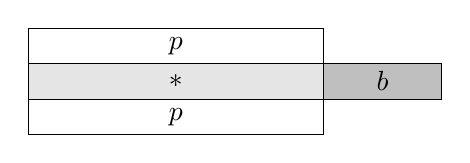
\begin{tikzpicture}[scale=1.5]

                    % Beam
                    \draw[fill=gray!20] (0,0) rectangle (2.5,0.3) node[midway] {$*$};
                    \draw[fill=gray!50] (2.5,0) rectangle (3.5,0.3) node[midway] {$b$};

                    % Piezoelectric patches
                    \draw[fill=white] (0, 0.3) rectangle (2.5, 0.6) node[midway] {$p$};
                    \draw[fill=white] (0, 0.0) rectangle (2.5, -0.3) node[midway] {$p$};

                \end{tikzpicture}

                \caption{Connection between piezoelectric patches and beam.}

            \end{figure}

        \end{column}

        \begin{column}{0.4\textwidth}

            \begin{equation}
                \begin{aligned}
                    EJ^*     & = E_b J_b + 2 E_p J_p       \\
                    \rho A^* & = \rho_b A_b + 2 \rho_p A_p
                \end{aligned}
            \end{equation}

        \end{column}

    \end{columns}

\end{frame}
% \input{src/02 -

\appendix

\begin{frame}[allowframebreaks]{References}
    \nocite{*}
    \bibliography{bibliography}
\end{frame}

\begin{frame}[standout]
    Questions?
\end{frame}

\begin{frame}[standout]
    Thank you!
\end{frame}

\end{document}